\begin{enumerate}

%exo2
\item  La contrainte vient de ce que $\arcsin$ est définie seulement dans $[-1,1]$. Notons $A(x) = \frac{2x}{1+x^2}$ et montrons que la fonction $f$ est définie dans $\R$ car
\begin{displaymath}
 \forall x \in \R,\; -1 \leq A(x) \leq 1.
\end{displaymath}
En effet
\begin{align*}
\frac{2x}{1+x^{2}}+1=\frac{(1+x)^{2}}{1+x^{2}}\geq 0 &\Rightarrow -1 \leq A(x)\\
\frac{2x}{1+x^{2}}-1=-\frac{(1-x)^{2}}{1+x^{2}}\geq 0 &\Rightarrow A(x) \leq 1. 
\end{align*}
Comme $\arcsin$ est continue dans $[-1,1]$, la fonction $f$ est également continue dans $\R$. En revanche $\arcsin$ n'est dérivable que dans l'ouvert et 
\begin{displaymath}
 A(x) = 1 \Leftrightarrow x = 1, \hspace{1cm} A(x) = -1 \Leftrightarrow x = -1.
\end{displaymath}
La fonction $f$ est donc dérivable seulement dans $\left] -\infty, -1\right[ {} \cup {}  \left] 1 , 1\left[  {} \cup  {} \right] 1 , -\infty\right[$.\newline
Remarque pour étudier la dérivabilité, il ne faut pas chercher à calculer la dérivée mais rappeler les domaines de dérivabilité des fonctions en jeu.\newline
Posons $\theta =\arctan x$, l'expression devient :
\begin{displaymath}
 \frac{2x}{1+x^{2}} = \frac{2\tan \theta }{1+\tan ^{2}\theta }
  = 2\tan \theta \cos ^{2}\theta =\sin 2\theta.
\end{displaymath}
Par cons{\'e}quent, $2\theta $ est un ant{\'e}c{\'e}dent de $\frac{2x}{1+x^{2}}$ pour $\sin $ mais, suivant $x$, il n'est pas forcément dans le bon intervalle ($\left[ -\frac{\pi}{2}, \frac{\pi}{2}\right] $) pour $\arcsin$. Présentons les cas dans un tableau
\begin{center}
\renewcommand{\arraystretch}{1.5}
\begin{tabular}{|c|c|c|c|} \hline
$x$       & $\left] -\infty, -1\right] $                  & $\left[ -1 , 1\right] $                        & $\left[ 1 , +\infty\right[ $                 \\ \hline
$\theta$  & $\left] -\frac{\pi}{2}, \frac{\pi}{4}\right]$ & $\left[ -\frac{\pi}{4}, \frac{\pi}{4}\right]$  & $\left[ \frac{\pi}{4}, \frac{\pi}{2}\right[$ \\ \hline
$2\theta$ & $\left] -\pi, \frac{\pi}{2}\right]$           & $\left[ -\frac{\pi}{2}, \frac{\pi}{2}\right]$  & $\left[ \frac{\pi}{2}, \pi \right[$          \\ \hline
$f(x)$    & $-\pi - 2\arctan x $                          & $2\arctan x$                                   & $\pi - 2 \arctan x$                          \\ \hline
\end{tabular}
\end{center}
On peut justifier les expressions par les remarques suivantes.
\begin{itemize}
\item  Si $x \geq 1$, alors $2\theta \in \left[ \frac{\pi }{2},\pi \right[ $ donc $\pi -2\theta \in \left] 0,\frac{\pi }{2}\right] $ a le m{\^e}me sinus que $2\theta$.
\item  Si $x \leq -1$, on conclut en remarquant que $f$ est impaire.
\begin{displaymath}
 \forall x \leq -1,\; f(x) = -f(-x) = -\left( \pi - 2 \arctan (-x)\right) = -\pi -\arctan x. 
\end{displaymath}

\end{itemize}
Une autre méthode consiste à dériver. 
\begin{multline*}
\forall x \in \R\setminus \left\lbrace  -1 , +1\right\rbrace, \;
f'(x) = \left( \frac{2}{1+x^2} - \frac{4x^2}{(1+x^2)^2}\right) \frac{1}{\sqrt{1-\frac{4x^2}{(1+x^2)^2}}}\\
= \left( \frac{2}{1+x^2} - \frac{4x^2}{(1+x^2)^2}\right) \frac{1+x^2}{\left|1-x^2\right|} 
= 2 \, \frac{1 - x^2}{\left|1-x^2\right|} \frac{1}{1 + x^2}.
\end{multline*}
On obtient une expression qui est au signe près la dérivée de $2\arctan$. On forme un tableau analogue et on calcule les constantes en prenant les valeurs en $-1$ et $1$.

%exo3
\item
\begin{enumerate}
\item Un nombre complexe admet un argument dans $\left] -\frac{\pi}{2}, \frac{\pi}{2}\right[$ si et seulement si sa partie réelle est strictement positive.

\item Nommons $A$ le complexe à étudier. Ses parties r{\'e}elles et imaginaires se calculent en multipliant par $e^{ia}-t$ le num{\'e}rateur et le d{\'e}nominateur. On obtient respectivement
\begin{displaymath}
 \frac{1-t^{2}}{1-2t\cos a+t^{2}}, \hspace{1cm} \frac{2t\sin a}{1-2t\cos a+t^{2}}.
\end{displaymath}
Comme $ -1 < t < 1$ et $1-2t\cos a+t^{2} = \left| e^{ia} -t\right|^2>0$, la partie r{\'e}elle est strictement positive. Comme on l'a rappelé dans la question a., cela entraine que $A$ admet un argument (nommons le $\theta$) dans $\left] -\frac{\pi }{2},+\frac{\pi }{2}\right[$. 
\item Montrons que le $N$ proposé par l'énoncé de cette question est en fait l'argument $\theta$ introduit dans la question précédente.
\begin{displaymath}
\left. 
\begin{aligned}
 \tan \theta = \frac{\sin \theta}{\cos \theta} = \frac{|A|\sin \theta}{|A|\cos \theta}
 = \frac{\Im(A)}{\Re(A)} = \frac{2t\sin a}{1-t^{2}}.\\
 \theta \in \left] -\frac{\pi }{2},+\frac{\pi }{2}\right[
\end{aligned}
\right\rbrace \Rightarrow
\theta = \arctan \frac{2t\sin a}{1-t^{2}}.
\end{displaymath}
D'autre part
\begin{displaymath}
\left. 
\begin{aligned}
 1-2t\cos a+t^{2} &= \left| 1-e^{-ia}\right| ^{2}\\
 1+2t\cos a+t^{2} &= \left| 1+e^{-ia}\right| ^{2}
\end{aligned}
\right\rbrace \Rightarrow
 |A| = \sqrt{\frac{1+2t\cos a+t^{2}}{1 - 2t\cos a+t^{2}}} = e^M.
\end{displaymath}
On en déduit
\begin{displaymath}
 e^{S} = e^M e^{iN} = |A| e^{i\theta} = A = \frac{e^{-ia}+t}{e^{-ia}-t}.
\end{displaymath}

\item Lorsque $t>1$, la partie r{\'e}elle de $A$ est n{\'e}gative. Par cons{\'e}quent, $N = \arctan \frac{2t\sin a}{1-t^{2}}$ n'est plus un argument de $A$ mais $N+\pi$ (qui a la même tangente) en est un. On en d{\'e}duit
\begin{displaymath}
 e^{S} = e^M e^{iN} = |A| e^{i N} = - |A| e^{i(N+\pi)}= - A = - \frac{e^{-ia}+t}{e^{-ia}-t}.
\end{displaymath}
\end{enumerate}


%exo4
\item Les fonctions $\arccos \circ \sin$ et $\arcsin \circ \cos$ sont définies dans $\R$. Nommons les respectivement $acs$ et $asc$.  Elles sont  $2\pi$-périodiques. On peut aussi préciser diverses transformation en utilisant les propriétés de cours de $\arccos$ et $\arcsin$.
\begin{align*}
 acs(x+\pi) = \arccos \circ \sin (x+\pi) = \arccos(-\sin(x)) &= \pi - acs(x)\\
 asc(x+\pi) = \arcsin \circ \cos (x+\pi) = \arcsin(-\cos(x)) &= - asc(x) \\
 acs(-x) = \arccos(-\sin x) &= \pi -acs(x) \\
 asc(-x) = \arcsin(cos x) &= asc(x). 
\end{align*}
On peut ainsi réduire le domaine d'étude à $\left[ 0 , \frac{\pi}{2}\right] $. 
\begin{displaymath}
 \forall x \in \left[ 0 , \frac{\pi}{2}\right],  
 \left. 
 \begin{aligned}
\frac{\pi}{2} -x &\in  \left[ 0 , \frac{\pi}{2}\right] \\
\cos\left( \frac{\pi}{2} -x\right) &= \sin x \\ 
\sin\left( \frac{\pi}{2} -x\right) &= \cos x 
 \end{aligned}
\right\rbrace \Rightarrow
 acs(x) = asc(x) = \frac{\pi}{2} -x
\end{displaymath}
\begin{figure}[h]
 \centering
 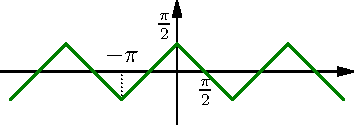
\includegraphics{./Celem4_1.pdf}
 % Celem4_1.pdf: 0x0 pixel, 0dpi, 0.00x0.00 cm, bb=
 \caption{Graphe de $\arcsin \circ \cos$.}
 \label{fig:Celem4_1}
\end{figure}
\begin{figure}[h]
 \centering
 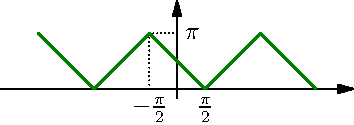
\includegraphics{./Celem4_2.pdf}
 \caption{Graphe de $\arccos \circ \sin$.}
 \label{fig:Celem4_2}
\end{figure}
Les graphes sont présentés en figures \ref{fig:Celem4_1} et \ref{fig:Celem4_2}.\newline
Les fonctions $\sin \circ \arccos$ et $\arccos \circ \sin$ sont très différentes. Elles sont définies dans le segment $\left[ -1,1\right]$ seulement. Elles sont égales entre elles et à la fonction $x \mapsto \sqrt{1-x^2}$ car les intervalles dans lesquels les fonctions $\arcsin$ et $\arccos$ prennent leurs valeurs permettent de lever l'ambiguité du signe devant la racine. Leur graphe est le demi-cercle unité. 
\begin{figure}[h]
 \centering
 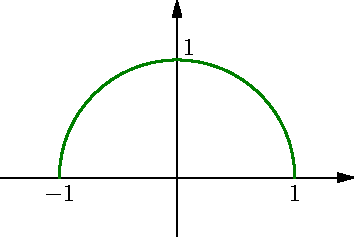
\includegraphics{./Celem4_3.pdf}
 \caption{Graphe de $\sin \circ \arccos$ et $\cos \circ \arcsin$.}
 \label{fig:Celem4_3}
\end{figure}


%exo8
\item Transformons le produit des deux coefficients du bin{\^o}me.
\begin{displaymath}
\binom{p+q}{k}\binom{p+q-k}{p-k} = \frac{(p+q)!(p+q-k)!}{k ! (p+q-k)! (p-k)!q!}
 = \frac{(p+q)! }{k ! (p-k)!q!}\frac{p!}{p!}
 = \binom{p+q}{p} \binom{p}{k} 
\end{displaymath}
On peut alors utiliser la formule du bin{\^o}me. La forme simple cherchée est donc
\begin{displaymath}
\binom{p+q}{p}\sum _{k=0}^{p}\binom{p}{k} = 2^{p} \binom{p+q}{p} 
\end{displaymath}

%exo10
\item La premi{\`e}re somme est la partie imaginaire de
\begin{multline*}
\sum _{k=0}^{n}\left(\frac{e^{ix}}{\cos x}\right)^k 
= \frac{1-\frac{e^{(n+1)ix}}{\cos^{n+1}x}}{1-\frac{e^{ix}}{\cos x}}
= \frac{1}{\cos^n x} \frac{\cos^{n+1}x - e^{(n+1)ix}}{\cos x - e^{ix}}\\
= \frac{1}{\cos^n x} \frac{\cos^{n+1}x - e^{(n+1)ix}}{- i\sin x}
= i\,\frac{\cos^{n+1}x - e^{(n+1)ix}}{\cos^{n}x \sin x}
\end{multline*}
soit
\begin{displaymath}
\frac{\cos x}{\sin x}-\frac{\cos(n+1)x}{\cos^{n}x\sin x} 
\end{displaymath}

La deuxi{\`e}me somme est la partie imaginaire de
\begin{displaymath}
 \left( 1+e^{ix}\right)^{n} = \left( 2\cos\frac{x}{2}e^{i\frac{x}{2}}\right)^{n}
\end{displaymath}
soit
\begin{displaymath}
2^{n}\cos^{n}\frac{x}{2}\sin\frac{nx}{2} 
\end{displaymath}


\end{enumerate}